\documentclass[aspectratio=169]{beamer}
\usetheme{Madrid}
\usefonttheme{structurebold}
\usefonttheme[onlymath]{serif}

\definecolor{BKTemplate}{rgb}{0.11765, 0.30588, 0.47451}
\usecolortheme[named=BKTemplate]{structure}
\setbeamercolor{title}{fg=BKTemplate,bg=} 
\setbeamertemplate{caption}[numbered]
\usepackage{array}
\usepackage[utf8]{inputenc}
\usepackage[T5]{fontenc}    % use T5 fonts for Vietnamese
\usepackage{url}            % simple URL typesetting
\usepackage{booktabs}       % professional-quality tables
\usepackage{amsfonts}       % blackboard math symbols
\usepackage{nicefrac}       % compact symbols for 1/2, etc.
\usepackage{microtype}      % microtypography
\usepackage{mathtools}
\usepackage{multicol}
\usepackage{comment}
\usepackage{forest}
\usepackage[linesnumbered, ruled]{algorithm2e}
\usepackage{algorithmic}
\usepackage{xcolor}
\usepackage{colortbl}
\usepackage{graphicx}
\usepackage{diagbox}
\usepackage{tikz}
\usepackage{subcaption}
% \captionsetup[subfigure]{labelsep=space}
\usepackage{amsmath}
\usepackage{dsfont}
\usepackage{stmaryrd}
\usepackage[style=authortitle,backend=bibtex]{biblatex}
\usepackage{array}
\usepackage{tabularx} % Khuyên dùng để bảng tự co dãn
% \addbibresource{thesiscite.bib}

\renewcommand{\footnotesize}{\tiny}
\newcommand{\mathbi}[1]{\boldsymbol{#1}}
\newtheorem{proposition}{Proposition}

%------------------------------------------------------------
%This block of code defines the information to appear in the
%Title page
\title[Đồ Án Chuyên Ngành HK251] %optional
{\vspace*{1cm}\\\textbf{\large BÁO CÁO ĐỒ ÁN CHUYÊN NGÀNH}}

\subtitle{\textbf{\Large PHÁT TRIỂN GAME FISHY-BUSINESS}}

\author[Nhóm Fishy-Business] % (optional)Hội Đồng: 14L
{\textbf{Hội Đồng:} 14L\\
\textbf{Mã Đề tài:} HK251-DAGD1-478 \\
\textbf{GVHD:} ThS. Vương Bá Thịnh\\
\vspace{0.2cm}
\textbf{SVTH:} Lê Ngọc Hiền (2211024)\\
Huỳnh Trần Học Đăng (2210731)\\
Nguyễn Mạnh Hùng (2211337)}
\vspace{-0.2cm}
\institute[HCMUT] % (optional)
{
  Khoa KH\&KT Máy tính
}
\date[Dec 2025] % (optional)
% {Tháng 12, 2025}

%End of title page configuration block
%------------------------------------------------------------

%------------------------------------------------------------
%The next block of commands puts the table of contents at the 
%beginning of each section and highlights the current section:
\AtBeginSection[]
{
  \begin{frame}
    \frametitle{Nội dung chính}
    \tableofcontents[currentsection]
  \end{frame}
}
%------------------------------------------------------------

\begin{document}

% The next statement creates the title page.
\setbeamertemplate{background canvas}{
	
\includegraphics[width=\paperwidth,height=\paperheight]{img/FrontBackground.pdf}
}

\begin{frame}[plain]
\titlepage
\end{frame}

% Set background for all pages
\setbeamertemplate{background canvas}{
	
\includegraphics[width=\paperwidth,height=\paperheight]{img/Background.pdf}
}

% \begin{frame}
% \frametitle{PHÂN CHIA CÔNG VIỆC}
% \begin{itemize}
%     \item \textbf{Lê Bá Khánh (2211509):} 
%     Xây dựng thuật toán Minimax với Alpha-Beta Pruning, thiết kế hàm đánh giá heuristic (Piece-Square Tables, Killer Instinct), triển khai Random Agent và Minimax Agent. (100\%)

%     \item \textbf{Nguyễn Mạnh Hùng (2211337):} 
%     Thuyết trình, thiết kế giao diện Pygame, xử lý sự kiện chuột/bàn phím, hiển thị bàn cờ và quân cờ, implement GameState class và tích hợp với python-chess. (100\%)

%     \item \textbf{Đoàn Trí Hùng (2211322):} 
%     Viết báo cáo, slide thuyết trình, phân tích kết quả thực nghiệm, tổng hợp tài liệu tham khảo, so sánh hiệu năng các Agent và đánh giá win rate. (100\%)

%     \item \textbf{Nguyễn Mạnh Tuấn (2213786):} 
%     Xử lý dữ liệu PGN, huấn luyện mô hình Deep Learning với TensorFlow, tối ưu hóa GPU acceleration, triển khai ML Agent với batch prediction. (100\%)
% \end{itemize}
% \end{frame}

%---------------------------------------------------------
%This block of code is for the table of contents after
%the title page
\begin{frame}
\frametitle{Nội dung chính}
\tableofcontents
\end{frame}




% =========================================================
\section{I. Giới Thiệu Đồ Án \& Mục Tiêu}
% =========================================================

% SLIDE 2: Bối Cảnh & Vấn Đề
\begin{frame}
\frametitle{Bối Cảnh \& Vấn Đề}
\begin{itemize}
    \item \textbf{Xu hướng hiện nay:} Trỗi dậy của dòng game "Suy luận xã hội" (\textit{Social Deduction}), điển hình như \textit{Among Us, Goose Goose Duck}.
    \item \textbf{Nhu cầu:} Người chơi khao khát sự kết nối, tương tác và "lừa lọc" vui vẻ với nhau.
    % \item \textbf{Tình hình thực tế:}
    % \begin{itemize}
    %     \item Các game \textit{Saboteur} trên thị trường chủ yếu là \textbf{2D tĩnh}.
    %     \item Thiếu không khí "tụ tập" và tương tác vật lý trong môi trường chơi.
    % \end{itemize}
    
    \item \textbf{Game bài trong Game:} Các trò chơi kinh điển như \textbf{Uno, Mèo nổ, Ma sói} đã chứng minh sức hút mãnh liệt khi được số hóa, tạo ra cộng đồng hàng triệu người chơi.
\end{itemize}
\vspace{0.5cm}
    Do đó, nhóm đã chọn đề tài phát triển một trò chơi dạng Suy luận xã hội và Party kết hợp với game bài.
\end{frame}

\begin{frame}
\frametitle{Các Game Tiêu Biểu Trên Thị Trường}
\begin{columns}
    \column{0.6\textwidth}
    \textbf{Sự Thành Công Của Dòng Game Social \& Party:}
    
    \begin{itemize}
        \item \textbf{Among Us (Social Deduction):}
        \begin{itemize}
            \item Trở thành hiện tượng toàn cầu với lối chơi suy luận đơn giản nhưng kịch tính.
            \item Thành công nhờ tạo ra các tình huống tương tác xã hội "dở khóc dở cười".
        \end{itemize}
         
    \end{itemize}
    \vspace{6em}

    \column{0.4\textwidth}
    \centering
    
    \begin{figure}
        \centering
        
\includegraphics[width=0.8\linewidth]{img/amongus.png}
        % \caption{Enter Caption}
        \label{fig:amongus}
    \end{figure}
\end{columns}
\end{frame}

\begin{frame}
\frametitle{Các Game Tiêu Biểu Trên Thị Trường}
\begin{columns}
    \column{0.6\textwidth}
    \textbf{Sự Thành Công Của Dòng Game Social \& Party:}
    
    \begin{itemize}
        \item \textbf{Among Us (Social Deduction):}
        \begin{itemize}
            \item Trở thành hiện tượng toàn cầu với lối chơi suy luận đơn giản nhưng kịch tính.
            \item Thành công nhờ tạo ra các tình huống tương tác xã hội "dở khóc dở cười".
        \end{itemize}
        
        \item \textbf{Liar's Bar (Psychological Tabletop):}
        \begin{itemize}
            \item Gây sốt nhờ kết hợp sự căng thẳng của trò chơi "Bluffing" với môi trường 3D sống động.
            \item Đạt thành công lớn trong việc mô phỏng áp lực tâm lý giữa những người chơi trực tiếp.
        \end{itemize}
        
    \end{itemize}
    \vspace{3em}

    \column{0.4\textwidth}
    \centering
    
    \begin{figure}
        \centering
        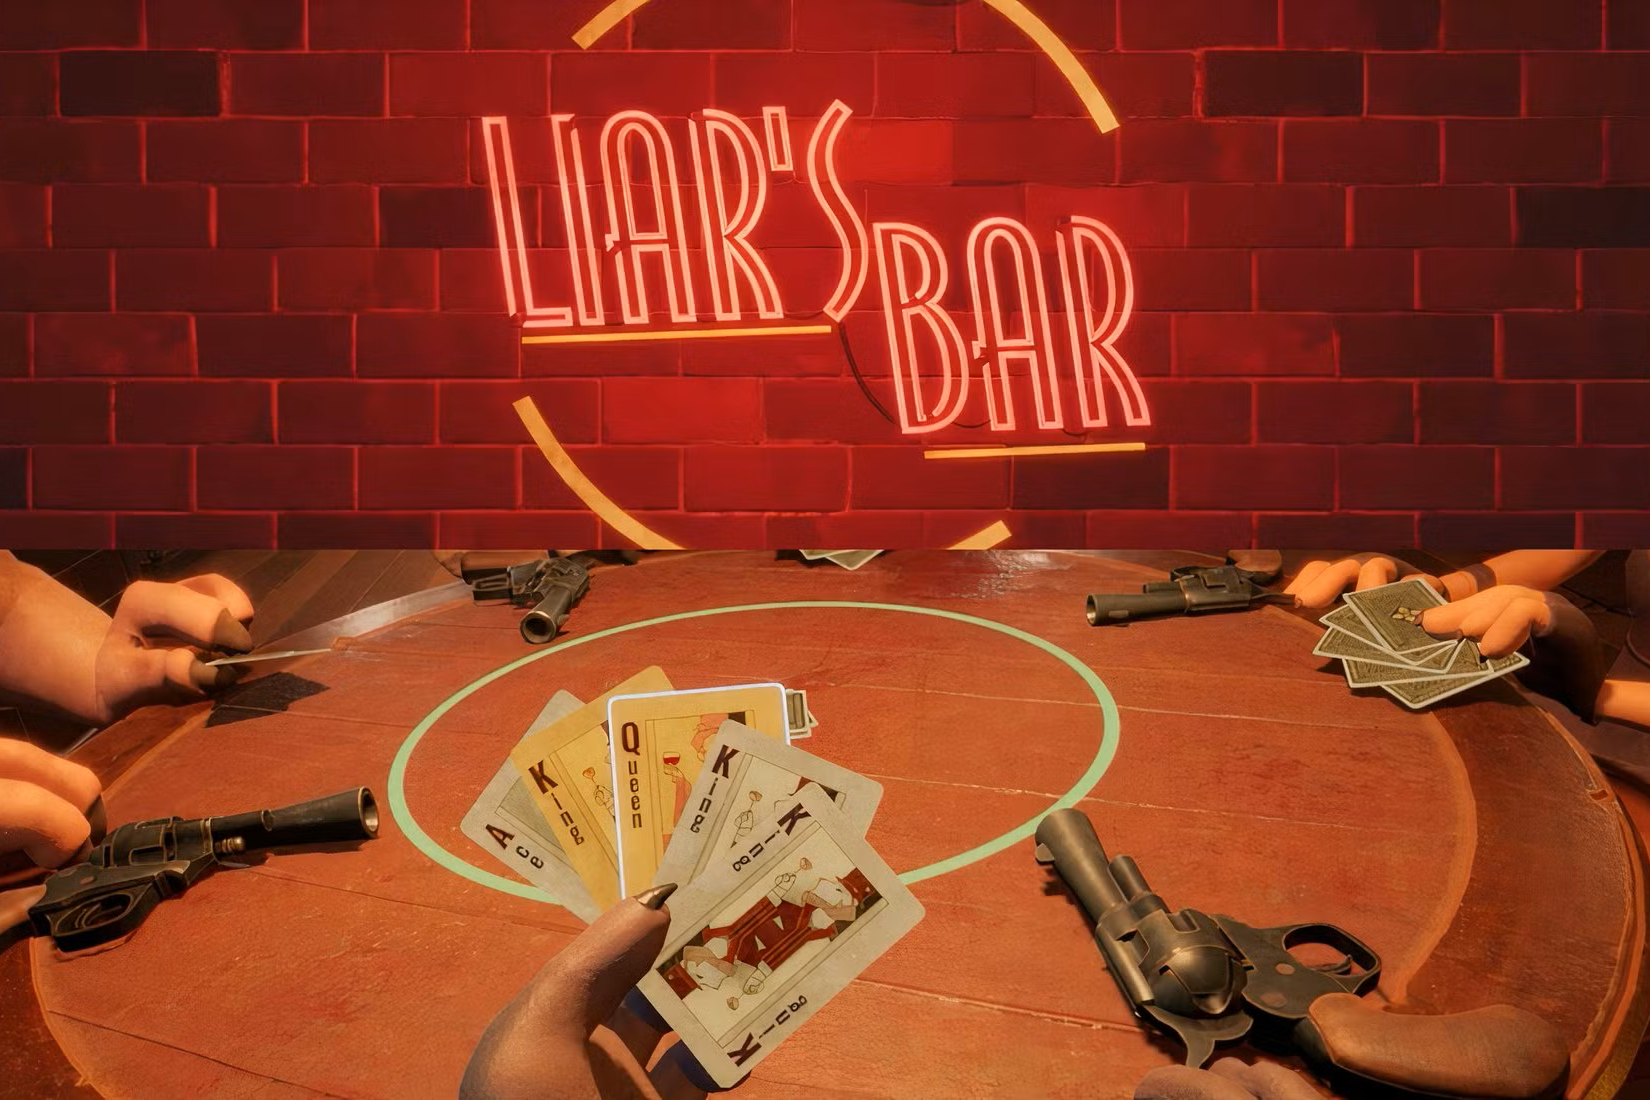
\includegraphics[width=0.9\linewidth]{img/liarsbar.png}
        % \caption{Enter Caption}
        \label{fig:liarsbar}
    \end{figure}
\end{columns}
\end{frame}


\begin{frame}
\frametitle{Các Game Tiêu Biểu Trên Thị Trường}
\begin{columns}
    \column{0.6\textwidth}
    \textbf{Sự Thành Công Của Dòng Game Social \& Party:}
    
    \begin{itemize}
        \item \textbf{Among Us (Social Deduction):}
        \begin{itemize}
            \item Trở thành hiện tượng toàn cầu với lối chơi suy luận đơn giản nhưng kịch tính.
            \item Thành công nhờ tạo ra các tình huống tương tác xã hội "dở khóc dở cười".
        \end{itemize}
        
        \item \textbf{Liar's Bar (Psychological Tabletop):}
        \begin{itemize}
            \item Gây sốt nhờ kết hợp sự căng thẳng của trò chơi "Bluffing" với môi trường 3D sống động.
            \item Đạt thành công lớn trong việc mô phỏng áp lực tâm lý giữa những người chơi trực tiếp.
        \end{itemize}
        
        \item \textbf{Party Animals (Highly Interactive Social):}
        \begin{itemize}
            \item Thu hút hàng triệu người chơi nhờ sự hài hước từ tương tác vật lý.
            \item Thành công nhờ đồ họa 3D bắt mắt và tính giải trí nhóm cực cao.
        \end{itemize}
    \end{itemize}

    \column{0.4\textwidth}
    \centering
    
    \begin{figure}
        \centering
        
\includegraphics[width=0.9\linewidth]{img/party-animals.png}
        % \caption{Enter Caption}
        \label{fig:animals}
    \end{figure}
\end{columns}
\end{frame}

\begin{frame}
\frametitle{Các Game Tiêu Biểu Trên Thị Trường}
\begin{columns}
    \column{0.6\textwidth}
    \textbf{Sự Thành Công Của Dòng Game Social \& Party:}
    
    \begin{itemize}
        \item \textbf{Among Us (Social Deduction):}
        \begin{itemize}
            \item Trở thành hiện tượng toàn cầu với lối chơi suy luận đơn giản nhưng kịch tính.
            \item Thành công nhờ tạo ra các tình huống tương tác xã hội "dở khóc dở cười".
        \end{itemize}
        
        \item \textbf{Liar's Bar (Psychological Tabletop):}
        \begin{itemize}
            \item Gây sốt nhờ kết hợp sự căng thẳng của trò chơi "Bluffing" với môi trường 3D sống động.
            \item Đạt thành công lớn trong việc mô phỏng áp lực tâm lý giữa những người chơi trực tiếp.
        \end{itemize}
        
        \item \textbf{Party Animals (Highly Interactive Social):}
        \begin{itemize}
            \item Thu hút hàng triệu người chơi nhờ sự hài hước từ tương tác vật lý.
            \item Thành công nhờ đồ họa 3D bắt mắt và tính giải trí nhóm cực cao.
        \end{itemize}
    \end{itemize}

    \column{0.4\textwidth}
    \centering
    
    \vspace{0.5em}
    \begin{block}{Chìa khóa thành công}
        Sự kết hợp giữa \textbf{Tương tác xã hội} + \textbf{Cảm xúc mạnh} + \textbf{Tính giải trí cao}.
    \end{block}
\end{columns}

\end{frame}

% SLIDE 3.1: Cảm Hứng: Saboteur
% \begin{frame}
% \frametitle{Saboteur}
% \begin{itemize}
%     \item \textbf{Luật chơi cốt lõi:}
%     \begin{itemize}
%         \item Phe \textbf{Thợ mỏ (Gold-Diggers)}: Cố gắng nối đường hầm từ điểm xuất phát đến kho báu.
%         \item Phe \textbf{Phá hoại (Saboteurs)}: Bí mật ngăn cản thợ mỏ mà không bị phát hiện.
%     \end{itemize}
%     \item \textbf{Cơ chế:} Đặt thẻ đường, dùng thẻ hành động (phá, sửa, xem map) và \textit{bluffing} (đánh lừa).
%     \item \textbf{Trang bị trong bộ Saboteur}
%     \begin{itemize}
%       \item 40 Thẻ đường (path cards): gồm 31 thẻ thông, 9 thẻ cụt
%       \item 27 Thẻ hành động (action cards)
%       \item 11 Thẻ vai trò (role cards)
%     \end{itemize}
% \end{itemize}
% \end{frame}

\begin{frame}
\frametitle{Cảm Hứng: Saboteur - Trò Chơi Suy Luận Xã Hội Cổ Điển}
\begin{columns}
    % Cột 1: Nội dung và Tương tác (0.55 width)
    \column{0.55\textwidth}
    \textbf{Tính Hấp Dẫn \& Tương Tác:}
    \begin{itemize}
        \item \textbf{Ẩn vai trò (Hidden Roles):} Người chơi không biết ai là Saboteur cho đến phút cuối.
        \item \textbf{Tương tác trực tiếp:} Dùng thẻ hành động để phá hoại công cụ của đối thủ hoặc sửa chữa cho đồng đội.
        \item \textbf{Cơ chế \textit{Bluffing}:} Khả năng đánh lừa, đổ lỗi và thuyết phục là chìa khóa chiến thắng.
    \end{itemize}
    
    % \textbf{Luật Chơi Cơ Bản:}
    % \begin{itemize}
    %     \item Phe \textbf{Thợ mỏ (Gold-Diggers)}: Cố gắng nối đường hầm từ điểm xuất phát đến kho báu.
    %     \item Phe \textbf{Phá hoại (Saboteurs)}: Bí mật ngăn cản thợ mỏ bằng cách đặt thẻ bế tắc hoặc phá hủy đường đi.
    % \end{itemize}
    
    \textbf{Đánh Giá Từ Cộng Đồng (BGG):}
    \begin{itemize}
        \item \textbf{Độ khó:} 1.3/5
        % (Rất dễ tiếp cận, luật chơi đơn giản).
        \item \textbf{Độ lừa lọc: Cao} 
        % \textit{Cực cao} – Linh hồn của trò chơi.
        \item \textbf{Thời gian chơi:} 30 - 45 phút 
        % (Nhanh, phù hợp cho tiệc tùng).
        \item \textbf{Số lượng người chơi:} 3 - 10 người 
        % (Tương tác càng cao khi càng đông).
        % \item \textbf{Độ hấp dẫn:} 7.0/10
        % (Trò chơi "nhập môn" kinh điển).
    \end{itemize}
    % Cột 2: Hình ảnh (0.45 width)
    \column{0.45\textwidth}
    \centering
    \begin{figure}
        \centering
        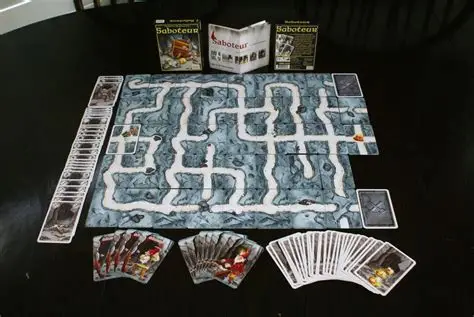
\includegraphics[width=0.9\linewidth]{img/saboteur.png}
        % \caption{Enter Caption}
        \label{fig:placeholder}
    \end{figure}

    % \captionof{figure}{Mô phỏng Board Game Saboteur}
\end{columns}
\end{frame}

% SLIDE 4: Giải Pháp: Fishy Business
\begin{frame}
\frametitle{Mục Tiêu: Fishy Business}
\begin{columns}
    \column{0.5\textwidth}
    \textbf{1. Hiện thực game}
    \begin{itemize}
        \item Số hóa toàn bộ luật chơi: chia bài, kiểm tra đường đi, tính điểm tự động.
        \item Loại bỏ sự rườm rà của việc thiết lập (setup) thủ công.
    \end{itemize}
    \vspace{0.8em} % Tăng khoảng cách một chút để thoáng bài
    \textbf{2. Môi trường 3D}
    \begin{itemize}
        \item Không gian Cabin 3D sống động, tối ưu hóa trải nghiệm thị giác.
        \item Người chơi có Avatar, có thể di chuyển và biểu cảm thời gian thực.
    \end{itemize}

    \column{0.5\textwidth}
    \textbf{3. Multiplayer}
    \begin{itemize}
        \item Kết nối nhiều người chơi thông qua mạng Network.
        \item Tích hợp Voice-Text Chat giúp giao tiếp và "biện minh" trực tiếp.
    \end{itemize}
    \vspace{0.8em}
    \textbf{4. Giải trí bổ trợ}
    \begin{itemize}
        \item Giải quyết "thời gian chết" bằng các hoạt động bên lề thú vị.
        \item Chơi nhạc cụ ảo (piano, guitar), thay đổi trang phục linh hoạt.
    \end{itemize}
\end{columns}
\end{frame}

% SLIDE 5: So Sánh Với Đối Thủ
% \begin{frame}
% \frametitle{Các Game Có Mặt Trên Thị Trường}
% \begin{table}
% \centering
% \begin{tabular}{|l|c|c|c|}
%     \hline
%     \textbf{Tiêu chí} & \textbf{Tabletop Simulator} & \textbf{Board Game Arena} & \textbf{Fishy Business (Project)} \\
%     \hline
%     \textbf{Nền tảng} & PC (Sandbox) & Web (2D) & PC (3D App) \\
%     \hline
%     \textbf{Luật chơi} & Thủ công (Tự tính) & Tự động & Tự động hoàn toàn \\
%     \hline
%     \textbf{Đồ họa} & 3D (Mô phỏng vật lý) & 2D Tĩnh & 3D Social Hub \\
%     \hline
%     \textbf{Tương tác} & Voice chat & Text chat & Avatar, Nhạc cụ, Voice \\
%     \hline
% \end{tabular}
% \end{table}
% \end{frame}

\input{sec/2}
\input{sec/3}
% =========================================================
\section{V. Tiến Độ Thực Hiện}
% =========================================================

% \begin{frame}
% \frametitle{Tiến Độ Thực Hiện}
% \begin{table}
% \centering
% \begin{tabular}{|c|l|}
%     \hline
%     \textbf{Thời gian} & \textbf{Công việc chính} \\
%     \hline
%     Tuần 1 & Lên kế hoạch từng giai đoạn, thiết kế UI tổng thể bằng figma \\
%     \hline
%     Tuần 2 - 4 & Hiện thực UI tổng thể, Lobby cơ bản, Model, Môi trường. \\
%     \hline
%     Tuần 5 - 8 & Hoàn thiện Core Gameplay \\
%     \hline
%     Tuần 8 - 10 & Chuyển Core Gameplay sang Multiplayer. \\
%     \hline
%     Tuần 11 - 12 & Tích hợp SFX, VFX, Voice Chat\\
%     \hline
%     Tuần 13 - 14 & Fix bug, Tinh chỉnh, Viết báo cáo, slides. \\
%     \hline
% \end{tabular}
% \end{table}
% \end{frame}

% SLIDE 17: Công việc đã đóng góp - Giai đoạn 1
\begin{frame}
\frametitle{Công việc đã đóng góp - Giai đoạn 1}
\begin{table}[H]
\centering
\renewcommand{\arraystretch}{1.2}
\small
\begin{tabular}{|c|l|}
\hline
\textbf{Sprint} & \textbf{Công việc chính} \\ \hline

Tuần 1--2 & Wireframe UI, tạo Lobby, tích hợp Player, bản đồ, camera, mô hình Card \\ \hline

Tuần 3--4 & Menu, phòng custom, cấu hình game, xử lý vị trí ngồi, chia/chọn bài \\ \hline

Tuần 5--6 & Hoàn thiện Lobby (kick player, quick match), triển khai dùng bài, camera \\ \hline

Tuần 7--8 & UI thay đổi thông tin, hoạt ảnh di chuyển, đồng bộ dữ liệu, sửa lỗi \\ \hline

Tuần 9--10 & Hệ thống âm thanh, Voice Chat, cải tiến ánh sáng, hiệu ứng VFX \\ \hline

Tuần 11--12 & Viết báo cáo tổng hợp, chuẩn bị slide thuyết trình \\ \hline

Tuần 13--14 & Sửa lỗi tồn đọng, nghiên cứu phát triển giai đoạn 2 \\ \hline

\end{tabular}
\end{table}
\end{frame}

% SLIDE 18: Công việc đã đóng góp - Giai đoạn 2
\begin{frame}
\frametitle{Công việc đã đóng góp - Giai đoạn 2}
\begin{table}[H]
\centering
\renewcommand{\arraystretch}{1.2}
\small
\begin{tabular}{|c|l|}
\hline
\textbf{Sprint} & \textbf{Công việc chính} \\ \hline

Tuần 1--2 & Lên kế hoạch chi tiết, thiết kế Figma, refactor code, vẽ diagram \\ \hline

Tuần 3--4 & Hiện thực UI gameplay mới, Day Night Phase, thẻ chức năng, ban vote \\ \hline

Tuần 5--6 & Fix volume, Push-to-talk, Emote, Voice Chat, Text Chat \\ \hline

Tuần 7--8 & Tooltip, hướng dẫn điều khiển, map mới, respawn player, VFX/SFX \\ \hline

Tuần 9--10 & Fix gameplay, quay video demo, cải tiến camera angle, setup itch.io \\ \hline

Tuần 11--12 & Thu thập phản hồi người dùng, hoàn thiện báo cáo, slide \\ \hline

\end{tabular}
\end{table}
\end{frame}

% SLIDE 19: Kế Hoạch Tiếp Theo
% \begin{frame}
% \frametitle{Kế Hoạch Tiếp Theo}
% \begin{table}[H]

% \centering
% \renewcommand{\arraystretch}{1.3}
% \begin{tabular}{|c|c|}
% \hline
% \textbf{Thời gian} & \textbf{Nội dung chính} \\ \hline

% Tuần 1--2 & Xây dựng Text Chat và hệ thống biểu cảm người chơi \\ \hline

% Tuần 3--4 & Cải thiện tương tác gameplay và trải nghiệm người chơi \\ \hline

% Tuần 5--6 & Thêm map mới, giao diện chọn map, tích hợp thêm SFX và VFX \\ \hline

% Tuần 7--8 & Chuyển sang mô hình Client--Server và phát triển board game mới \textit{Liar Bar!} \\ \hline

% Tuần 9--10 & Tối ưu hiệu suất mạng và nâng cấp giao diện người dùng (UI) \\ \hline

% Tuần 11--12 & Chuẩn bị bản build và phát hành trên \textit{itch.io} \\ \hline

% Tuần 13--14 & Thu thập phản hồi người chơi và tổng kết dự án \\ \hline

% \end{tabular}
% \end{table}

% \end{frame}




\setbeamertemplate{footline}{}

\begin{frame}
    \centering
    \vspace{1cm}
    \textbf{\Huge{- THE END - }}\\
    \vspace{0.2cm}
    \textit{\Large{Cảm ơn thầy/cô đã lắng nghe phần trình bày của nhóm em}}\\
    \vspace{15pt}
    % \begin{columns}
    %     \begin{column}{0.6\textwidth}
    %         \centering
    %         \includegraphics[width=0.8\textwidth]{img/paper.jpg}
    %     \end{column}
    %     \begin{column}{0.4\textwidth}
    %         \centering
    %        Q \& A
    %     \end{column}
    % \end{columns}
\end{frame}


\end{document}